\documentclass[compress,xcolor=table]{beamer}

% Packages
\usepackage[english]{babel}
\usepackage[utf8]{inputenc}
\usepackage[T1]{fontenc}
\usepackage{datetime}
\usepackage{multicol}

% Possible options of the package (add/remove below in \usetheme call):
%  - nosectionpages: no pages between sections
%  - flama: use flama font, requires xelatex/lualatex + the font to compile
%  - compressminiframes: put the heading list bullets indications pages on 1 line
\usetheme[compressminiframes]{sorbonne}

% Title page
\title{\Huge Formalisation and\\Evaluation of\\Properties for\\Consequentialist\\Machine Ethics}

\foottitle{} % optional, printed at the bottom of the slides, by default same as title, can be useful to rewrite when title has a newline for example
\subtitle{} % optional subtitle
\date{\formatdate{16}{05}{2024}}
\author{Titouan Guerin}
% \institute{LIP6 - Sorbonne Université} % Optional

% Biblatex
\usepackage[backend=bibtex, style=authoryear, citestyle=authoryear]{biblatex}
\bibliography{library.bib}
\renewcommand*{\bibfont}{\footnotesize}


%%%%
%% BEGIN OF SLIDES
%%%%
\setbeamerfont{section in head/foot}{size={\fontsize{5}{3}}}
\begin{document}

\begin{frame}[plain]
	\titlepage
	\setcounter{framenumber}{0}
\end{frame}

\section{Introduction}

\begin{frame}{Contexte}

    \begin{block}{Motivation}
        \begin{itemize}
            \item AI systems increasingly make decisions that impact humans’ lives (self-driving cars)
            \item Need to follow ethical principles
        \end{itemize}
    \end{block}
    \pause
    \begin{block}{Problem}
        \begin{itemize}
            \item Existing approaches lack rigorous justification and formal comparison.
        \end{itemize}
    \end{block}
\end{frame}

\begin{frame}{Ethics}
    There are 3 main approaches to ethics:
    \pause
    \begin{itemize}
        \item consequentialism: judges actions only based on their \textbf{consequences}
        \item deontology: notion of \textbf{duty} to determine whether an action/ sequence of actions is right or wrong
        \item virtue ethics: uses agent’s \textbf{character and intention} to determine the appropriateness of their actions
    \end{itemize}
    \pause
    \begin{block}{}
        We will focus on \textbf{consequentialism} because it is the dominant approach to machine ethics so far and the focus of this paper.
    \end{block}
\end{frame}

\begin{frame}{Problematique}
    \begin{alertblock}{Question}
    How can machine ethics approaches properly validate their formalisation of ethical principles and determine the most appropriate principle(s) to apply in a given situation?
    \end{alertblock}
    \pause
    \begin{block}{Contributions}
        \begin{itemize}
            \item Framework to evaluate ethical principles systematically,
            \item Define formal principles and properties for decision-making.
        \end{itemize}
    \end{block}
\end{frame}

\begin{frame}{Running example}
    \textit{We have available to us exactly \textbf{one smart robot}, designed to assist in decision-making when “incidents” occur. A \textbf{fire just started} on the top floor of a building \textbf{full of employees}. The robot needs to \textbf{keep everyone safe} but also to \textbf{minimise the damage by extinguishing the fire}. It has three choices:}
    \begin{itemize}
        \item \textit{(a) rush into the source of the fire and extinguish it,} 
        \item \textit{(b) personally help the evacuation of employees until everyone is safe,}
        \item \textit{(c) trigger the fire alarm while calling the fire department.}
    \end{itemize}

    \textbf{What should it do?}
\end{frame}

\section{Situation Calculus}

\begin{frame}{Situation Calculus}
    \begin{block}{What is it?}
    \begin{itemize}
        \item Formal framework to model and reason about changing environments 
        \pause
        \item Compute what happens if an agent performs a sequence of actions
    \end{itemize}
    \end{block}
    \pause
    Lets define the framework!
\end{frame}

\begin{frame}{Definitions}
    \begin{block}{Fluents}
        \textbf{What they are:} Properties of the world that can change over time, \\
        \textbf{Example:} "The building is on fire", "Employees are safe", "The fire is extinguished", \\
        \textbf{Formal notation:} $F(\vec{x},s)$ means "property $F$ with arguments $\vec{x}$ is true in situation $s$." 
    \end{block}
    \pause
    \begin{block}{Situations}
        \textbf{What they are:} Snapshots of the world at a given time, including the history of actions that led to it, \\
        
        \textbf{Example:} 
        \begin{itemize}
            \item $s_0$: Initial situation (building on fire, employees inside)
            \item $do(a,s)$: The situation after performing action $a$ in situation $s$.
        \end{itemize}

        \textbf{Formal notation:} $do([evac,extg],s_0)$ means the situation after evacuating and then extinguishing the fire.
    \end{block}
\end{frame}

\begin{frame}{Definitions}
    \begin{block}{Actions}
        \textbf{What they are:} Things that change the world, \\
        \textbf{Example:} $evac$ (evacuate employees), $extg$ (extinguish fire), $call$ (call the fire department).
    \end{block}
    \pause
    \begin{block}{Action Preconditions}
        \textbf{What they are:} Conditions that must be true for an action to be possible.\\
        \textbf{Example:} To $extg$, the robot must be near the fire source.\\
        \textbf{Formal notation:} $Poss(a(\vec{x}),s) \equiv \pi_a(\vec{x}, s)$ means "action $a$ is possible in situation $s$ if $\pi_a$ is true."
    \end{block}
\end{frame}

\begin{frame}{Definitions}
    \begin{block}{ Effect Axioms}
        \textbf{What they are:} Rules that describe how actions change fluents.\\
        \begin{itemize}
            \item Positive effect: $F$ becomes true after $a$.
            \item Negative effect: $F$ becomes false after $a$.
        \end{itemize}

        \textbf{Example:}\\
        \begin{itemize}
            \item $do(evac,s)$ makes "employees are safe" true.
            \item $do(extg,s)$ makes "building is on fire" false.
        \end{itemize}
        
        \textbf{Formal notation:}\\
        \begin{itemize}
            \item $\gamma_F^+(\vec{x}, a, s) \rightarrow F(\vec{x}, do(a, s))$ (positive effect)
            \item $\gamma_F^-(\vec{x}, a, s) \rightarrow \neg F(\vec{x}, do(a, s))$ (negative effect)
        \end{itemize}
    \end{block}
\end{frame}

\begin{frame}{Definitions}
    \begin{block}{ Successor State Axiom}
        \textbf{What it is:} A rule that fully describes how a fluent changes after an action,\\
        \textbf{Example:} If $extg$ is performed, "building is on fire" becomes false, and all other fluents stay the same unless changed,\\
        \textbf{Formal notation:}
$F(\vec{x}, do(a, s)) \equiv \gamma_F^+(\vec{x}, a, s) \vee (F(\vec{x}, s) \wedge \neg \gamma_F^-(\vec{x}, a, s))$
    \end{block}
    \pause
    \begin{block}{Plans}
        \textbf{What they are:} Sequences of actions,\\
        \textbf{Example:} $\pi = [evac, extg, call]$, \\
        \textbf{Formal notation:} $do(\pi, s_0)$ is the situation after executing plan $\pi$ from $s_0$.
    \end{block}
\end{frame}

\begin{frame}{Updated Example}
    \textit{Consider an initial state of our example where the building is on fire and all employees are inside. The robot has options to extinguish the fire ($extg$), evacuate all employees ($evac$), and call the fire department ($call$). The employees will get injured if not evacuated immediately and the building will become more damaged the longer it is not extinguished.}\\
    \pause
    \begin{block}{}
    Let's try and give some examples using the previous definition!    
    \end{block}
    
\end{frame}

\begin{frame}{Examples}
    In $s_0$, we can say that:
    \begin{itemize}
        \item $OnFire(s0)$: True (the building is on fire),
        \item $EmployeesSafe(s0)$: False (employees are not safe),
        \item $FireExtinguished(s0)$: False (the fire is not extinguished),
    \end{itemize}
    \pause
    And some action preconditions could be:
    \begin{itemize}
        \item $Poss(extg,s) \equiv OnFire(s)$: The robot can extinguish the fire only if the building is on fire,
        \item $Poss(evac,s) \equiv \neg EmployeesSafe(s)$: The robot can evacuate employees only if they are not already safe.
    \end{itemize}
    \pause
    And one positive effect axiom could be:
    \begin{itemize}
        \item $\gamma^{+}_{FireExtinguished}(extg,s) \rightarrow FireExtinguished(do(extg,s))$ which means that performing the extinguish action in $s$ always results in $FireExtinguished$ to become True.
    \end{itemize}
    
\end{frame}

\section{Formalisation of Ethical Principles}

\begin{frame}{Definition}
    \begin{alertblock}{Overview}
        Objective here is not to achieve a \textbf{goal}, but rather to see 
        if a plan satisfies an \textbf{ethical principle}. \\
    \end{alertblock}
    \pause
    \begin{block}{Goodness}
        We define a plan as \textbf{ethically permissable} based on its \textit{goodness}.\\
        We introduce the function $goodness(state(s))$ which returns a $value$.\\
        We also introduce $harmful(\varphi)$ which is true if $\varphi$ is a harmful fluent.\\
    \end{block}
    \pause
    We simplify the notation for \textit{admissible} plans and goodness:
    \begin{itemize}
        \item $state(\pi) = state(do(\pi, s_0))$
        \item $goodness(\pi) = goodness(state(\pi))$
    \end{itemize}
\end{frame}

\begin{frame}{Admissibility}
    \begin{alertblock}{Ethical Admissibility}
        We define a plan $\pi$ as \textbf{ethically admissible} if it is both possible 
        and satisfies an ethical principle.
    \end{alertblock}
    The paper defines 5 ethical principles: \textbf{utilitarianism}, \textbf{hedonism}, \textbf{no new harm}, \textbf{remove harm} and \textbf{harm avoidance}.\\
    Let's define them formally!
\end{frame}

\begin{frame}{Ethical Principles}
    \small
    \begin{block}{Utilitarianism}
        It focuses on bringing the greatest good to the greatest number of people:
        $$
        \mathcal{E}\mathcal{P}_{util}(\Pi, s_0) =
        \{ \pi \in \Pi \mid goodness(\pi) \geq goodness(\pi')
        \text{ for all } \pi' \in \Pi \}
        $$
    \end{block}
    \pause
    Example: \\
    If $goodness([evac,extg])>goodness([extg,call])$, then $[evac,extg]$ is  ethically permissible.

    \tiny
    \underline{Note:} $\mathcal{E}\mathcal{P}$ stands for ethical permissibility function.

\end{frame}

\begin{frame}{Ethical Principles}
    \small
    \begin{block}{Hedonism}
        Based on the overall consequences that it produces, a direct interpretation of consequentialism: any
        plan is ethically permissible if it has more goodness at the
        end state compared to the initial state.
        $$
        \mathcal{E}\mathcal{P}_{hedon}(\Pi, s_0) =
        \{ \pi \in \Pi \mid goodness(\pi) \geq goodness(\emptyset)\}
        $$
    \end{block}
    \pause
    Example: \\
    If $goodness([evac]) \geq goodness(\emptyset)$, then $[evac]$ is ethically permissible.
\end{frame}

\begin{frame}{Ethical Principles}
    \small
    \begin{block}{No New Harm}
    It dictates that a plan should not cause any new harm, so an agent should not
    be directly(or actively) responsible for any harm. This also means that we tolerate 
    a harm that is unavoidable.       
    $$
    \begin{aligned}
    \mathcal{E}\mathcal{P}_{\text{nnHarm}}(\Pi, s_0)
    &= \{ \pi \in \Pi \mid \text{for all } \varphi,\ 
    \text{if } harmful(\varphi) \text{ and } state(s_0) \not\vdash \varphi, \\
    &\quad \text{then } \big(
        state(\pi) \not\vdash \varphi
        \ \text{or for all } \pi' \in \Pi,\ 
        state(\pi') \vdash \varphi
    \big) \}
    \end{aligned}
    $$

    \end{block}
    \pause
    Explanation:\\
    For every harmful predicate $\varphi$,

If $\varphi$ is not true in the initial state ($state(s_0) \not\vdash \varphi$),
Then $\varphi$ must not become true after executing $\pi$ ($state(\pi) \not\vdash \varphi$),
unless $\varphi$ becomes true after every admissible plan (for all $\pi' \in \Pi$, $state(\pi') \vdash \varphi$), i.e unavoidable.

\end{frame}

\begin{frame}{Remove Harm}
    \small
    \begin{block}{Remove Harm}
        A plan is ethically permissible if it removes existing harm in the initial situation. 
        It requires the agent to mitigate harm whenever possible.
        $$
    \begin{aligned}
    \mathcal{E}\mathcal{P}_{\text{nnHarm}}(\Pi, s_0)
    &= \{ \pi \in \Pi \mid \text{for all } \varphi,\ 
    \text{if } harmful(\varphi) \text{ and } state(s_0) \vdash \varphi, \\
    &\quad \text{then } \big(
        state(\pi) \not\vdash \varphi
        \ \text{or for all } \pi' \in \Pi,\ 
        state(\pi') \vdash \varphi
    \big) \}
    \end{aligned}
    $$
    \end{block}
    \pause
    Explanation:\\
    For every harmful predicate $\varphi$, if it is found in the initial state ($state(s_0) \vdash \varphi$),
    then an acceptable plan $\pi$ must remove it, or every possible plan must have it at the end (so unavoidable).
    
\end{frame}

\begin{frame}{Harm Avoidance}
    \small
    \begin{block}{Harm Avoidance}
        A plan is ethically permissible if it minimises the amount of harm in the end state.
        $$
        \begin{aligned}
        \mathcal{E}\mathcal{P}_{\text{harmAvoid}}(\Pi, s_0)
        &= \{ \pi \in \Pi \mid 
        \text{for all } \varphi, \text{ if } harmful(\varphi), \\
        &\quad \text{then } \big( state(\pi) \not\vdash \varphi 
        \ \text{or for all } \pi' \in \Pi,\ state(\pi') \vdash \varphi \big) \}
        \end{aligned}
        $$
    \end{block}
    \pause
    Explanation:\\
    For every harmful predicate $\varphi$, an acceptable plan $\pi$ must ensure that $\varphi$ is not true in the end state,
    or every possible plan must have it at the end (so unavoidable). It is a combination of the two previous principles.
\end{frame}

\begin{frame}{Example}
    Let's define that the most important thing is to keep the employees safe. So we define the world as:\\
    \begin{itemize}
        \item $inside(emp, do(a, s)) \equiv inside(emp, s) \land a \neq evac$
        \item $onfire(do(a, s)) \equiv onfire(s) \land a \neq extg$
        \item $injured(emp, do(a, s)) \equiv inside(emp, s) \land onfire(s) \land a \neq evac$
        \item $injured'emp, do(a, s)) \equiv injured(emp, s) \land a \neq evac \land inside(emp, s) \land onfire(s)$
    \end{itemize}
    Here $emp$ is the employee and $injured(emp)$ the penatly of letting someone get injured. 
    $injured'(emp)$ means even more damage to an employee.\\
\end{frame}

\begin{frame}{Example}
    According to our previous definitions, we model the goodness function as:
    \begin{multicols}{2}
    \tiny
    \begin{itemize}
        \item $goodness([call]) = -10$
        \item $goodness([extg]) = -10$
        \item $goodness([evac]) = 0$
        \item $goodness([call, evac]) = -10$
        \item $goodness([evac, call]) = 0$
        \item $goodness([extg, call]) = -20$
        \item $goodness([call, extg]) = -20$
        \item $goodness([evac, extg]) = 0$
        \item $goodness([extg, evac]) = -10$
        \item $goodness([call, evac, extg]) = -10$
        \item $goodness([evac, call, extg]) = 0$
        \item $goodness([extg, call, evac]) = -20$
        \item $goodness([call, extg, evac]) = -20$
        \item $goodness([evac, extg, call]) = 0$
        \item $goodness([extg, evac, call]) = -10$
    \end{itemize}
    \end{multicols}
    Therefore, with the goodness of initial state set to 0, we have:\\
    $$
    \begin{aligned}
    \mathcal{E}\mathcal{P}_{util}(\Pi, s_0) 
    &= \{ [evac], [evac, call], [evac, call, extg],\\
     [evac, extg], [evac, extg, call] \} \\
    \mathcal{E}\mathcal{P}_{hedon}(\Pi, s_0) 
    &= \{ \} 
    \end{aligned}
    $$
\tiny
\underline{Note:} Hedonism returns empty set because no plan has a goodness strictly 
greater than the initial state, which has a goodness of 0.
\end{frame}

\section{Formalisation of Properties}

\begin{frame}{Definition}
    \begin{alertblock}{Overview}
        We want to define properties that can be used to \textbf{evaluate and compare} ethical principles.\\
        Based on which properties are verified, we can make an \textbf{educated choice} on what principle to follow
        according to the context/situation.
    \end{alertblock}
    \pause
    The authors define 8 properties which are directly derived from the principles we just saw.\\
    7 more are presented, and are derived from properties found in social choice theory (we will define what this means later).
\end{frame}

\begin{frame}{Ethical Properties}
    \begin{block}{Consequential Equivalence}
        We define this as moral actions that produce "good" consequences. It also states that two plans
        with the same consequences should be considered equally ethical.
    \end{block}
    If $\pi \in \mathcal{EP}(\Pi, s_0)$ and $state(do(\pi, s_0)) = state(do(\pi', s_0))$, then $\pi' \in \mathcal{EP}(\Pi, s_0)$, for all $\pi' \in \Pi$
    
    Example: \\
    Suppose $[evac,extg]$ and $[extg,evac]$ both result in the same final state (employees safe, fire extinguished).
    If $[evac,extg] \in \mathcal{EP}(\Pi, s_0)$, then $[extg,evac] \in \mathcal{EP}(\Pi, s_0)$.

\end{frame}

\begin{frame}{Ethical Properties}
    \begin{block}{Maximal Welfare}
        An ethically permissible plan must produce at least as much goodness as any other plan that is ethically admissible.
    \end{block}
    if $\pi \in \mathcal{EP}(\Pi, s_0)$, then for all $\pi' \in \Pi$, $goodness(\pi) \geq goodness(\pi')$

    Example: \\
    If $[evac,extg] \in \mathcal{EP}(\Pi, s_0)$ and $[call]$ is a plan (not yet determined if ethical or not), 
    then for $[call]$ to be ethically permissible, it must have at least as much goodness as $[evac,extg]$.
\end{frame}

\begin{frame}{Ethical Properties}
    \begin{block}{Aggregationism}
        If a plan is ethically permissible and another plan is even better (i.e greater goodness), 
        then the better plan must also be ethically permissible.
    \end{block}
    if $\pi \in \mathcal{EP}(\Pi, s_0)$ and $goodness(\pi') \geq goodness(\pi)$, \\
    then $\pi' \in \mathcal{EP}(\Pi, s_0)$ and for all $\pi' \in \Pi$,
\end{frame}

\begin{frame}{Ethical Properties}
    \begin{block}{Independance}
        The permissibility of a plan should not depend on irrelevant alternatives. 
        If a plan is permissible in a larger set, 
        it should remain permissible in any subset containing it.       
    \end{block}
    $\mathcal{EP}(\Pi, s_0) \cap \Pi' \subseteq \mathcal{EP}(\Pi', s_0)$

    Intuition:\\
    If a plan $\Pi$ is ethically permissible, and we consider the intersection between this plan and another set of plans $\Pi'$, 
    then this intersection should be a subset of the ethically permissible plans in $\Pi'$.
\end{frame}

\begin{frame}{Ethical Properties}
    \begin{block}{Beneficence}
        A permissible plan must be better than doing nothing. 
        In other words, the overall goodness at the end of the plan
        must be better than the overall goodness at the beginning of the plan.
    \end{block}
    If $\pi \in \mathcal{EP}(\Pi, s_0)$, then $goodness(\pi) > goodness(\emptyset)$.

    \vfill

    \tiny
    \underline{Note:} this property and Independance are closely tied to Hedonism. 
\end{frame}

\begin{frame}{Ethical Properties}
    \begin{alertblock}{New Notations}
        We define the following terms for the next three properties:
        \begin{itemize}
            \item $harms(\pi) = \{ \varphi \mid state(\pi) \vdash \varphi \wedge harmful(\varphi) \}$ 
            \item $newState(\pi) = \{ F(\vec{x}) \mid F(\vec{x}, do(\pi, s_0)) \wedge \neg F(\vec{x}, s_0) \}$
            \item $oldState(\pi) = \{ F(\vec{x}) \mid F(\vec{x}, do(\pi, s_0)) \wedge F(\vec{x}, s_0) \}$
        \end{itemize}
    \end{alertblock}

    \begin{block}{Positive Responsibility}
        This property defines that ethical permissibility should be determined only by the 
        new state such actions produce. Together with Harmlessness, this property is closely aligned
        with the No New Harm principle.
    \end{block}

    If $\pi \in EP(\Pi, s_0)$ and $newState(\pi) = newState(\pi')$, \\
    then $\pi' \in EP(\Pi, s_0)$, for all $\pi' \in \Pi$.
    
\end{frame}

\begin{frame}{Ethical Properties}
    \begin{block}{Negative Responsibility}
    The property is requiring that an ethically plan should eliminate existing harm
    or maintain the current good, and is closely aligned with the Remove Harm principle. I.e we want the agent
    to be responsible for inaction or maintaining harm. 
    \end{block}
    If $\pi \in \mathcal{EP}(\Pi, s_0)$ and $oldState(\pi) = oldState(\pi')$, \\
    then $\pi' \in \mathcal{EP}(\Pi, s_0)$, for all $\pi' \in \Pi$.
\end{frame}

\begin{frame}{Ethical Properties}
    \begin{block}{Harmlessness}
        This property focuses on the harm of a plan. We should only allow plans that aim to prevent harm,
        and so the harm at the end of the plan determines its ethical permissibility.
    \end{block}
   If $\pi \in \mathcal{EP}(\Pi, s_0)$ and $harms(\pi') \subseteq harms(\pi)$, \\
   then $\pi' \in \mathcal{EP}(\Pi, s_0)$, for all $\pi' \in \Pi$.
\end{frame}



\begin{frame}{Social Choice Properties}
    \begin{block}{Overview}
    Social choice theory designs protocols to select the best outcomes from preferences or choices.  
    \begin{itemize}
        \item Aggregating individual preferences into collective decisions,
        \item Analyzing voting systems,
        \item Investigating choice functions.
    \end{itemize}  
    The paper presents seven social choice properties to ensure \(\mathcal{EP}\) is robust and consistent.
    \end{block}
\end{frame}

\begin{frame}{Social Choice Properties}
    \begin{block}{Consistency Preservation (cp)}
        This property ensures that if there are any admissible plans, at least one must be ethically permissible. It guarantees that a decision is always made, even in dilemmas.
    \end{block}
    If \(\Pi \neq \emptyset\), then \(\mathcal{EP}(\Pi, s_0) \neq \emptyset\).
    \pause
    \begin{block}{Iteration (it)}
        This property requires that applying the ethical permissibility function twice (or more) does not change the result. It ensures stability in decisions.
    \end{block}
    \(\mathcal{EP}(\mathcal{EP}(\Pi, s_0), s_0) = \mathcal{EP}(\Pi, s_0)\).
\end{frame}


\begin{frame}{Social Choice Properties}
    \begin{block}{Cut (c)}
        This property states that if you remove some impermissible plans from \(\Pi\), the permissibility of the remaining plans does not change. It ensures robustness when the set of plans is reduced.
    \end{block}
    If \(\mathcal{EP}(\Pi, s_0) \subseteq \Pi' \subseteq \Pi\), then \(\mathcal{EP}(\Pi, s_0) \subseteq \mathcal{EP}(\Pi', s_0)\).
    \pause
    \begin{block}{Aizerman (aiz)}
        This property ensures that if you restrict the set of plans to a subset \(\Pi'\) that includes all permissible plans, the result does not change. It guarantees that adding back previously rejected plans does not affect the permissibility of the kept plans.
    \end{block}
    If \(\mathcal{EP}(\Pi, s_0) \subseteq \Pi' \subseteq \Pi\), then \(\mathcal{EP}(\Pi', s_0) \subseteq \mathcal{EP}(\Pi, s_0)\).

    \tiny
    \underline{Note:} these two are tightly related, and refer to contextual blindness.
\end{frame}

\begin{frame}{Social Choice Properties}
    \begin{block}{Chernoff (ch)}
        This property requires that if you shrink the set of plans (\(\Pi' \subseteq \Pi\)), the permissible plans in \(\Pi'\) must include those that were permissible in \(\Pi\). It ensures fairness when the set of plans is reduced.
    \end{block}
    If \(\Pi' \subseteq \Pi\), then \(\mathcal{EP}(\Pi, s_0) \cap \Pi' \subseteq \mathcal{EP}(\Pi', s_0)\).
    \pause
    \begin{block}{Sen (s)}
        This property states that if a plan \(\pi\) is permissible in both \(\Pi\) and \(\Pi'\), then it must be permissible in their intersection \(\Pi \cap \Pi'\). It ensures consistency across different contexts.
    \end{block}
    If \(\mathcal{EP}(\Pi, s_0) \cap \mathcal{EP}(\Pi', s_0) \neq \emptyset\), then \(\mathcal{EP}(\Pi \cap \Pi', s_0) \subseteq \mathcal{EP}(\Pi, s_0) \cap \mathcal{EP}(\Pi', s_0)\).

\end{frame}


\begin{frame}{Social Choice Properties}
    \begin{block}{Arrow (iia)}
        This property, also known as Independence of Irrelevant Alternatives, requires that if a subset \(\Pi'\) of plans includes some permissible plans from \(\Pi\), then the permissible plans in \(\Pi'\) are exactly those. It ensures that the permissibility of a plan depends only on how it compares to other available plans.
    \end{block}
    If \(\Pi' \subseteq \Pi\) and \(\mathcal{EP}(\Pi, s_0) \cap \Pi' \neq \emptyset\), then \(\mathcal{EP}(\Pi, s_0) \cap \Pi' = \mathcal{EP}(\Pi', s_0)\).
\end{frame}


\section{Results}

\begin{frame}{Results}
    \begin{block}{Recap}
        \textit{Principles} are \textbf{filters}, which directly select which plans 
        are permissible based on their ethical criteria.\\
        \textit{Properties} are tools to \textbf{evaluate and compare principles}:
        how a principle behaves or what it guarantees.

    \end{block}
    \small
    Example:
    \begin{itemize}
        \item Maximal Welfare: "Does this principle always select plans that maximize goodness?"
        \item Harmlessness: "Does this principle avoid causing unnecessary harm?"
        \item Consistency Preservation: "Does this principle always select at least one plan, even in dilemmas?"
    \end{itemize}

\end{frame}

\begin{frame}{Results}
    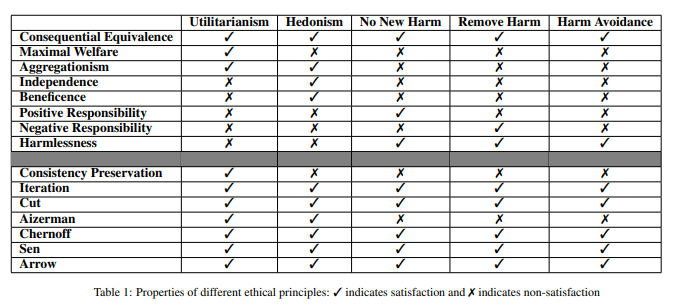
\includegraphics[width=\textwidth,height=0.9\textheight,keepaspectratio]{images/table1.png}    
\end{frame}

\begin{frame}{Utilitarianism}
    \begin{block}{Key Idea}
        Utilitarianism focuses on \textbf{maximizing overall welfare}, \\
        even if it means accepting some harm or less-than-ideal outcomes. \\
        \begin{center}
            \textit{"The greatest good for the greatest number."}
        \end{center}
    \end{block}
    \tiny
    \begin{block}{Consequential Equivalence}
            Plans with the same outcome are treated equally.\\
            $[evac, extg]$ and $[extg, evac]$ are both permissible if they result in the same state (employees safe, fire extinguished).
    \end{block}

    \begin{block}{Maximal Welfare}
        A permissible plan must produce at least as much goodness as any other plan.\\
        If $[evac, extg]$ has $goodness = 10$ and $[call]$ has $goodness = 5$, \\
        only $[evac, extg]$ is permissible.
    \end{block}

    \begin{block}{Aggregationism}
        If a plan is permissible and another plan is even better, 
        the better plan must also be permissible.\\

        If $[evac]$ is permissible ($goodness = 7$), \\
        $[evac, extg]$ ($goodness = 10$) must also be permissible.
    \end{block}

\end{frame}

\begin{frame}{Hedonism}
    \begin{block}{Key Idea and Contrast}
        Hedonism focuses on \textbf{ensuring a net benefit} compared to doing nothing. \\
        \begin{center}
            \textit{"A plan must be better than inaction."}
        \end{center}
    \end{block}
    \tiny
    \begin{block}{Consequential Equivalence \& Aggregationism}
        Same as Utilitarianism.
    \end{block}

    \begin{block}{Independence}
        Permissibility does not depend on irrelevant alternatives.\\
        If $[evac]$ is permissible in $\Pi = \{[evac], [extg], [call]\}$, \\
        it remains permissible in $\Pi' = \{[evac], [extg]\}$.
    \end{block}

    \begin{block}{Beneficence}
        Permissible plans must improve the initial state.\\
        $[call]$ ($goodness = -2$) is not permissible if the initial state has $goodness = 0$.
    \end{block}

\end{frame}

\begin{frame}{No New Harm}
    \begin{block}{Key Idea}
        No New Harm focuses on \textbf{avoiding new harm}, \\
        even if it means tolerating existing harm. \\
        \begin{center}
            \textit{"Do not produce a harm if it can be avoided."}
        \end{center}
    \end{block}
    \tiny
    \begin{block}{Consequential Equivalence}
        Plans with the same outcome are treated equally.\\
        $[evac, call]$ and $[call, evac]$ are both permissible if they result in the same state (no new harm introduced).
    \end{block}

    \begin{block}{Positive Responsibility}
        A permissible plan must not introduce new harm.\\
        If $[evac]$ avoids new harm but $[extg]$ risks injuries, \\
        only $[evac]$ is permissible.
    \end{block}

    \begin{block}{Harmlessness}
        If a plan causes less harm than a permissible plan, \\
        it must also be permissible.\\
        If $[evac]$ is permissible, $[evac, call]$ (less risky) must also be permissible.
    \end{block}
\end{frame}

\begin{frame}{Remove Harm}
    \begin{block}{Key Idea}
        Remove Harm focuses on \textbf{eliminating existing harm}, \\
        even if it means tolerating some new harm. \\
        \begin{center}
            \textit{"Eliminate a pre-existing harm if possible."}
        \end{center}
    \end{block}
    \tiny
    \begin{block}{Consequential Equivalence}
        Plans with the same outcome are treated equally.\\
        $[extg, call]$ and $[call, extg]$ are both permissible if they result in the same state (existing harm removed).
    \end{block}

    \begin{block}{Negative Responsibility}
        A permissible plan must eliminate existing harm.\\
        If $[extg]$ removes the fire but $[call]$ doesn't, \\
        only $[extg]$ is permissible.
    \end{block}

    \begin{block}{Harmlessness}
        If a plan causes less harm than a permissible plan, \\
        it must also be permissible.\\
        If $[extg]$ is permissible, $[extg, evac]$ (removes more harm) must also be permissible.
    \end{block}
\end{frame}

\begin{frame}{Harm Avoidance}
    \begin{block}{Key Idea and Contrast}
        Harm Avoidance focuses on \textbf{avoiding all avoidable harms}, \\
        both new and existing. \\
        \begin{center}
            \textit{"Avoid all avoidable harms!"}
        \end{center}
        \begin{itemize}
            \item Stricter than No New Harm and Remove Harm.
            \item May reject all plans if none avoid all harms.
        \end{itemize}
    \end{block}
    \tiny
    \begin{block}{Consequential Equivalence}
        Plans with the same outcome are treated equally.\\
        $[evac, extg]$ and $[extg, evac]$ are both permissible if they result in the same state (all harms avoided).
    \end{block}

    \begin{block}{Harmlessness}
        A permissible plan must avoid all avoidable harms.\\
        If $[evac]$ leaves fire burning and $[extg]$ risks injuries, \\
        neither may be permissible.
    \end{block}
\end{frame}

\begin{frame}{Social Choice Properties: Universally Satisfied}
    \begin{block}{Key Idea}
        These properties are satisfied by \textbf{all five principles}:
    \end{block}
    \tiny
    \begin{block}{Iteration}
        Applying the ethical permissibility function twice doesn't change the result.\\
        \textit{Example:} If $[evac, extg]$ is permissible, re-applying $\mathcal{EP}$ won't exclude it.
    \end{block}

    \begin{block}{Cut}
        Removing impermissible plans doesn't affect permissible ones.\\
        \textit{Example:} If $[evac]$ is permissible in $\Pi$, it remains permissible in $\Pi' = \{[evac], [extg]\}$.
    \end{block}

    \begin{block}{Chernoff}
        Shrinking the set of plans preserves permissibility.\\
        \textit{Example:} If $[evac]$ is permissible in $\Pi$, it remains permissible in $\Pi' = \{[evac]\}$.
    \end{block}

    \begin{block}{Sen}
        Plans permissible in both sets must be permissible in their intersection.\\
        \textit{Example:} If $[evac]$ is permissible in both $\Pi$ and $\Pi'$, it's permissible in $\Pi \cap \Pi'$.
    \end{block}

    \begin{block}{Arrow}
        Permissibility depends only on available plans.\\
        \textit{Example:} If $[evac]$ is permissible in $\Pi = \{[evac], [extg]\}$, its permissibility doesn't change if $[call]$ is added.
    \end{block}
\end{frame}

\begin{frame}{Consistency Preservation: Utilitarianism Only}
    \begin{block}{Key Idea}
        Only Utilitarianism satisfies this property:
    \end{block}
    \tiny
    \begin{block}{Definition}
        If there are any admissible plans, at least one must be permissible.\\
        If $\Pi \neq \emptyset$, then $\mathcal{EP}(\Pi, s_0) \neq \emptyset$.
    \end{block}

    \begin{block}{Why Utilitarianism?}
        Always selects the "least bad" option, even if all plans are harmful.\\
        \textit{Example:} In $\Pi = \{[evac], [extg]\}$ where both cause harm, Utilitarianism picks the one with less harm.
    \end{block}

    \begin{block}{Why Not Others?}
        Harm-based principles may reject all plans if all cause harm.\\
        \textit{Example:} No New Harm might reject both $[evac]$ and $[extg]$ if both introduce new harm.
    \end{block}
\end{frame}

\begin{frame}{Aizerman: Only Hedonism and Utilitarianism}
    \begin{block}{Key Idea}
        Only these Utilitarianism and Hedonism satisfy Aizerman.
    \end{block}
    \tiny
    \begin{block}{Definition}
        Restricting plans to a subset containing all permissible plans doesn't change results.\\
        If $\mathcal{EP}(\Pi, s_0) \subseteq \Pi' \subseteq \Pi$, then $\mathcal{EP}(\Pi', s_0) \subseteq \mathcal{EP}(\Pi, s_0)$.
    \end{block}

    \begin{block}{Why Utilitarianism?}
        Focuses on maximal welfare, unaffected by adding back rejected plans.\\
        \textit{Example:} If $[evac]$ is permissible in $\Pi$, it remains so in $\Pi' = \{[evac], [do\ nothing]\}$.
    \end{block}

    \begin{block}{Why Hedonism?}
        Only requires improvement over inaction, unaffected by additional options.\\
        \textit{Example:} If $[evac]$ improves over inaction, it remains permissible even if $[do\ nothing]$ is added.
    \end{block}

    \begin{block}{Why Not Others?}
        Harm-based principles may change permissibility when new options are added.\\
        \textit{Example:} Harm Avoidance might reject $[evac]$ if $[do\ nothing]$ is added (avoids all harm).
    \end{block}
\end{frame}

\begin{frame}{Conclusion: Novel Contributions}
    \begin{block}{Key Innovations}
        \begin{itemize}
            \item \textbf{First formal framework} for consequentialist machine ethics using situation calculus.
            \item \textbf{Two major contributions}:
            \begin{itemize}
                \item Formalized 5 ethical principles 
                \item Defined 15 properties 
            \end{itemize}
            \item \textbf{Proved property satisfaction} for each principle, enabling precise characterization.
            \item \textbf{Bridged philosophy and AI} by translating ethical theories into computational logic.
        \end{itemize}

        \tiny
        Proofs are available here: bit.ly/3JUVrU9
    \end{block}

    \begin{block}{Why This Matters}
        \begin{itemize}
            \item Enables \textbf{rigorous analysis} of ethical AI systems.
            \item Provides \textbf{toolkit} to validate and compare ethical approaches.
            \item Facilitates \textbf{transparent, explainable} ethical decision-making in AI.
        \end{itemize}
    \end{block}
\end{frame}

\begin{frame}{Future Directions and Impact}
    \begin{block}{Conclusions}
        \begin{itemize}
            \item No single principle is perfect - each satisfies some properties but not others.
            \item \textbf{Trade-offs} must be considered based on application context.
        \end{itemize}
    \end{block}

    \begin{block}{Future Research Opportunities}
        \begin{itemize}
            \item Extend to \textbf{deontological and hybrid} approaches.
            \item Incorporate \textbf{uncertainty} in ethical reasoning.
            \item Study \textbf{prioritization of principles} in complex scenarios.
            \item Develop \textbf{tooling} for practical implementation.
            \item Validate with \textbf{real-world case studies}.
        \end{itemize}
    \end{block}
\end{frame}

\section{Thank You}

\section{Appendix}

\begin{frame}{Full Example Definition}
    \begin{block}{Fluents}
        \begin{itemize}
            \item $OnFire(s)$
            \item $EmployeesSafe(s)$
            \item $FireExtinguished(s)$
            \item $FireDepartmentCalled(s)$
            \item $BuildingDamaged(s)$
            \item $EmployeesInjured(s)$
        \end{itemize}
    \end{block}

    \begin{block}{Actions}
    \begin{itemize}
        \item $extg$
        \item $evac$
        \item $call$
    \end{itemize}
    \end{block}
\end{frame}

\begin{frame}{Full Example Definition}
\small
    \begin{block}{Initial Definition}
        \begin{itemize}
            \item $OnFire(s_0)=True$
            \item $EmployeesSafe(s_0)=False$
            \item $FireExtinguished(s_0)=False$
            \item $FireDepartmentCalled(s_0)=False$
            \item $BuildingDamaged(s_0)=False$
            \item $EmployeesInjured(s_0)=False$
        \end{itemize}
    \end{block}

    \begin{block}{Action Precondition Axioms}
        \begin{itemize}
            \item $Poss(extg,s) \equiv OnFire(s)$
            \item $Poss(evac,s) \equiv \neg EmployeesSafe(s)$
            \item $Poss(call,s) \equiv \neg FireDepartmentCalled(s)$
        \end{itemize}
    \end{block}
\end{frame}

\begin{frame}
\small
    \begin{block}{Positive Effect Axioms}
        \begin{itemize}
            \item $\gamma_{FireExtinguished}^+(extg, s) \rightarrow FireExtinguished(do(extg,s))$
            \item $\gamma_{EmployeesSafe}^+(evac, s) \rightarrow EmployeesSafe(do(evac,s))$
            \item $\gamma_{FireDepartmentCalled}^+(call, s) \rightarrow FireDepartmentCalled(do(call,s))$
        \end{itemize}
    \end{block}

    \begin{block}{Negative Effect Axioms}
        \begin{itemize}
            \item $\gamma_{OnFire}^-(extg, s) \rightarrow \neg OnFire(do(extg,s))$
            \item $\gamma_{BuildingDamaged}^-(call, s) \rightarrow \neg BuildingDamaged(do(call,s))$
            \item $\gamma_{EmployeesInjured}^-(evac, s) \rightarrow \neg EmployeesInjured(do(evac,s))$
        \end{itemize}
    \end{block}
\end{frame}

\end{document}

